\documentclass[12pt]{article}
\usepackage[utf8]{inputenc}
\usepackage[catalan]{babel}
\usepackage{amsmath, amssymb, amsfonts}
\usepackage{geometry}
\usepackage{fancyhdr}
\usepackage{tikz}
\usetikzlibrary{matrix, calc}
\usepackage{tcolorbox}
\usepackage[colorlinks=true, linkcolor=blue]{hyperref}

\setlength{\headheight}{15pt} % Augmentem l'altura de l'encapçalament

% Definicions de geometria
\geometry{a4paper, left=2cm, right=2cm, top=2.5cm, bottom=2.5cm}

% Configuració de l'encapçalament i peu de pàgina
\pagestyle{fancy}
\fancyhf{}
\fancyhead[L]{Matemàtiques 2n Batxillerat}
\fancyhead[R]{Sistemes d'equacions}
\fancyfoot[L]{\href{mailto:orodri11@xtec.cat}{orodri11@xtec.cat}}
\fancyfoot[R]{\thepage}

% Estils per a quadres
\newtcolorbox{concept}[1][]{colback=blue!5!white, colframe=blue!75!black, fonttitle=\bfseries, title=Concepte, #1}
\newtcolorbox{exemple}[1][]{colback=green!5!white, colframe=green!75!black, fonttitle=\bfseries, title=Exemple, #1}
\newtcolorbox{exercici}[1][]{colback=yellow!5!white, colframe=yellow!75!black, fonttitle=\bfseries, title=Exercici, #1}

\begin{document}

% Portada
\begin{titlepage}
    \centering
    {\Huge \textbf{Sistemes d'equacions \\ 2n Batxillerat} \par}
    \vspace{1cm}
    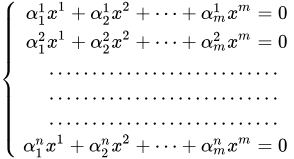
\includegraphics[width=0.5\textwidth]{Sistemes.png}
    \vspace{1cm}
    \tableofcontents
\end{titlepage}

\newpage

% Secció 1: Sistemes d'equacions
\section{Sistemes d'equacions}

\subsection{Introducció}
\begin{concept}
Un sistema d'equacions lineals és un conjunt d'\(m\) equacions amb \(n\) incògnites que han de complir-se simultàniament. Es pot expressar de forma general:
\[
\begin{cases}
a_{11}x_1 + a_{12}x_2 + \cdots + a_{1n}x_n = b_1 \\
a_{21}x_1 + a_{22}x_2 + \cdots + a_{2n}x_n = b_2 \\
\vdots \\
a_{m1}x_1 + a_{m2}x_2 + \cdots + a_{mn}x_n = b_m
\end{cases}
\]
\end{concept}

\subsection{Classificació dels sistemes}
\begin{concept}
Segons el nombre de solucions:
\begin{itemize}
    \item \textbf{Sistema compatible determinat (SCD):} Té una única solució.
    \item \textbf{Sistema incompatible (SI):} No té solució.
    \item \textbf{Sistema compatible indeterminat (SCI):} Té infinites solucions.
\end{itemize}
\end{concept}

\subsection{Mètodes de resolució}
\begin{concept}
Els mètodes principals per resoldre sistemes són:
\begin{itemize}
    \item Substitució
    \item Igualació
    \item Reducció
\end{itemize}
\end{concept}

\subsection*{Exemples resolts}
\begin{exemple}
\textbf{Sistema compatible determinat (SCD):}
\[
\begin{cases}
x + 2y + z = 6 \\
2x - y + 3z = 14 \\
3x + 4y - z = 8
\end{cases}
\]

\end{exemple}

\begin{exemple}
Resolució per reducció:\\

1. Eliminem \(x\) de la segona i tercera equacions:
\[
\begin{aligned}
(2x - y + 3z) - 2(x + 2y + z) &= 14 - 12 \\
-5y + z &= 2 \\
(3x + 4y - z) - 3(x + 2y + z) &= 8 - 18 \\
-2y - 4z &= -10
\end{aligned}
\]
2. Simplifiquem el nou sistema amb dues equacions:
\[
\begin{cases}
-5y + z = 2 \\
-2y - 4z = -10
\end{cases}
\]
3. Eliminem \(y\) i resolvem per \(z\):
\[
-2(-5y + z) + (-2y - 4z) = -4 + (-10) \quad \Rightarrow \quad -14z = -14 \quad \Rightarrow \quad z = 1
\]
Substituïm \(z = 1\) i trobem \(y\) i \(x\):
\[
-5y + 1 = 2 \quad \Rightarrow \quad y = -\frac{1}{2}, \quad x = 3
\]
Solució: \(x = 3, y = -\frac{1}{2}, z = 1\).
\end{exemple}

\subsection*{Exercicis proposats}
\begin{exercici}
Resol el sistema següent per reducció:
\[
\begin{cases}
2x + y + z = 7 \\
3x - y + 2z = 14 \\
x + 4y - z = 3
\end{cases}
\]
\end{exercici}

\begin{exercici}
Resol el sistema següent:
\[
\begin{cases}
x - 2y + 3z = 5 \\
2x + y - z = 4 \\
3x + 4y + z = 10
\end{cases}
\]
\end{exercici}

\newpage

\section{El mètode de Gauss}

\subsection{Matriu del sistema i matriu ampliada}
\begin{concept}
Un sistema de \(m\) equacions amb \(n\) incògnites té associades dues matrius:
\begin{itemize}
    \item \textbf{Matriu del sistema:} És la matriu \(M\) formada pels coeficients de les incògnites.
    \item \textbf{Matriu ampliada:} És la matriu \(M'\), que s'obté afegint a la dreta de \(M\) una columna amb els termes independents.
\end{itemize}

Per exemple, considerem el sistema:
\[
\begin{cases}
a_{11}x_1 + a_{12}x_2 + \dots + a_{1n}x_n = b_1 \\
a_{21}x_1 + a_{22}x_2 + \dots + a_{2n}x_n = b_2 \\
\vdots \\
a_{m1}x_1 + a_{m2}x_2 + \dots + a_{mn}x_n = b_m
\end{cases}
\]

La seva matriu del sistema \(M\) i matriu ampliada \(M'\) són:
\[
M = 
\begin{bmatrix}
a_{11} & a_{12} & \dots & a_{1n} \\
a_{21} & a_{22} & \dots & a_{2n} \\
\vdots & \vdots & \ddots & \vdots \\
a_{m1} & a_{m2} & \dots & a_{mn}
\end{bmatrix}, \quad
M' = 
\begin{bmatrix}
a_{11} & a_{12} & \dots & a_{1n} & b_1 \\
a_{21} & a_{22} & \dots & a_{2n} & b_2 \\
\vdots & \vdots & \ddots & \vdots & \vdots \\
a_{m1} & a_{m2} & \dots & a_{mn} & b_m
\end{bmatrix}
\]
\end{concept}

\subsection{Mètode de Gauss}
\begin{concept}
El mètode de Gauss consisteix a transformar la matriu ampliada \(M'\) en una matriu escalonada mitjançant operacions elementals, que són:
\begin{itemize}
    \item Multiplicar una fila per un escalar no nul.
    \item Afegir o restar un múltiple d'una fila a una altra fila.
    \item Intercanviar l'ordre de dues files.
\end{itemize}

L'objectiu és obtenir una matriu en forma escalonada, a partir de la qual es poden trobar les solucions mitjançant substitució regressiva.
\end{concept}

\subsection{Classificació dels sistemes}
\begin{concept}
Segons el resultat del mètode de Gauss, podem classificar els sistemes en:
\begin{itemize}
    \item \textbf{Sistema compatible determinat (SCD):} Té una única solució. Es produeix quan totes les incògnites tenen valors determinats.
    \item \textbf{Sistema incompatible (SI):} No té solució. Es produeix quan apareix una equació inconsistent, com \(0 = c\) (on \(c \neq 0\)).
    \item \textbf{Sistema compatible indeterminat (SCI):} Té infinites solucions. Es produeix quan una o més variables queden lliures.
\end{itemize}
\end{concept}

\subsection*{Exemples resolts}
\begin{exemple}
\textbf{Sistema Compatible Determinat (SCD):}
\[
\begin{cases}
x + y + z = 6 \\
2x - y + 3z = 14 \\
3x + 4y - z = 8
\end{cases}
\]

1. Escriu la matriu ampliada:
\[
M' =
\begin{bmatrix}
1 & 1 & 1 & 6 \\
2 & -1 & 3 & 14 \\
3 & 4 & -1 & 8
\end{bmatrix}
\]

2. Fes \(F_2 \to F_2 - 2F_1\) i \(F_3 \to F_3 - 3F_1\):
\[
\begin{bmatrix}
1 & 1 & 1 & 6 \\
0 & -3 & 1 & 2 \\
0 & 1 & -4 & -10
\end{bmatrix}
\]

3. Fes \(F_3 \to F_3 + \frac{1}{3}F_2\):
\[
\begin{bmatrix}
1 & 1 & 1 & 6 \\
0 & -3 & 1 & 2 \\
0 & 0 & -\frac{11}{3} & \frac{-2}{3}
\end{bmatrix}
\]

4. Simplifica \(F_3\) i troba les solucions per substitució regressiva:
\[
z = -\frac{2}{11}, \quad y = 2, \quad x = 4
\]
\end{exemple}

\begin{exemple}
\textbf{Sistema Compatible Indeterminat (SCI):}
\[
\begin{cases}
x + y + z = 4 \\
2x + 3y + z = 7 \\
x + 2y + 2z = 5
\end{cases}
\]

1. Escriu la matriu ampliada:
\[
M' =
\begin{bmatrix}
1 & 1 & 1 & 4 \\
2 & 3 & 1 & 7 \\
1 & 2 & 2 & 5
\end{bmatrix}
\]

2. Fes \(F_2 \to F_2 - 2F_1\) i \(F_3 \to F_3 - F_1\):
\[
\begin{bmatrix}
1 & 1 & 1 & 4 \\
0 & 1 & -1 & -1 \\
0 & 1 & 1 & 1
\end{bmatrix}
\]

3. Fes \(F_3 \to F_3 - F_2\):
\[
\begin{bmatrix}
1 & 1 & 1 & 4 \\
0 & 1 & -1 & -1 \\
0 & 0 & 2 & 2
\end{bmatrix}
\]

4. Simplifica \(F_3\) dividint per 2:
\[
\begin{bmatrix}
1 & 1 & 1 & 4 \\
0 & 1 & -1 & -1 \\
0 & 0 & 1 & 1
\end{bmatrix}
\]

5. Substitució regressiva:
\begin{align*}
z &= \lambda \\
y - z &= -1 \quad \Rightarrow \quad y = \lambda - 1 \\
x + y + z &= 4 \quad \Rightarrow \quad x = 1 - 2\lambda \\
\lambda &\in \mathbb{R}
\end{align*}
\end{exemple}


\begin{exemple}
\textbf{Sistema Incompatible (SI):}
\[
\begin{cases}
x + y + z = 3 \\
2x + 2y + 2z = 6 \\
x + y + z = 5
\end{cases}
\]

\end{exemple}

\begin{exemple}
1. Escriu la matriu ampliada:
\[
M' =
\begin{bmatrix}
1 & 1 & 1 & 3 \\
2 & 2 & 2 & 6 \\
1 & 1 & 1 & 5
\end{bmatrix}
\]

2. Fes \(F_2 \to F_2 - 2F_1\) i \(F_3 \to F_3 - F_1\):
\[
\begin{bmatrix}
1 & 1 & 1 & 3 \\
0 & 0 & 0 & 0 \\
0 & 0 & 0 & 2
\end{bmatrix}
\]

3. La tercera fila indica \(0 = 2\), una contradicció.

Per tant, el sistema és incompatible i no té solució.
\end{exemple}


\subsection*{Exercicis proposats}
\begin{exercici}
Resol el sistema següent utilitzant el mètode de Gauss:
\[
\begin{cases}
2x + y - z = 3 \\
x + 3y + 2z = 7 \\
3x - 2y + z = 4
\end{cases}
\]
\end{exercici}

\begin{exercici}
Resol el sistema i classifica'l:
\[
\begin{cases}
x - y + 2z = 5 \\
3x + y - z = 10 \\
2x + 4y - 3z = 6
\end{cases}
\]
\end{exercici}

\newpage

\section{Teorema de Rouché-Frobenius}

\subsection{Teorema de Rouché-Frobenius}
\begin{concept}
El \textbf{teorema de Rouché-Frobenius} estableix que un sistema d'equacions lineals \(A \cdot X = B\), amb una matriu de coeficients \(A\) de dimensió \(m \times n\), té solució si i només si el rang de la matriu del sistema \(A\) és igual al rang de la matriu ampliada \(A'\):
\[
\text{rang}(A) = \text{rang}(A')
\]

A més, el teorema ens permet classificar els sistemes segons les seves solucions:
\begin{itemize}
    \item Si \( \text{rang}(A) = \text{rang}(A') = n \): El sistema és \textbf{compatible determinat} (SCD), té una solució única.
    \item Si \( \text{rang}(A) = \text{rang}(A') < n \): El sistema és \textbf{compatible indeterminat} (SCI), té infinites solucions.
    \item Si \( \text{rang}(A) \neq \text{rang}(A') \): El sistema és \textbf{incompatible} (SI), no té solució.
\end{itemize}
\end{concept}

\subsection{Sistemes homogenis}
\begin{concept}
Un sistema d'equacions lineals és \textbf{homogeni} quan els termes independents són tots zero, és a dir:
\[
A \cdot X = 0
\]

Les propietats dels sistemes homogenis són:
\begin{itemize}
    \item Sempre són \textbf{compatibles}, ja que la solució trivial (\(X = 0\)) satisfà el sistema.
    \item Si \( \text{rang}(A) = n \), el sistema només té la solució trivial (\(X = 0\)).
    \item Si \( \text{rang}(A) < n \), el sistema té infinites solucions (és compatible indeterminat).
\end{itemize}
\end{concept}

\subsection*{Exemples resolts}
\begin{exemple}
\textbf{Exemple 1:} Determinar si el sistema és compatible i classificar-lo:
\[
\begin{cases}
x + y + z = 3 \\
x + 2y + z = 4 \\
2x + 3y + 2z = 7
\end{cases}
\]

\end{exemple}

\begin{exemple}
1. Matriu del sistema:
\[
A =
\begin{bmatrix}
1 & 1 & 1 \\
1 & 2 & 1 \\
2 & 3 & 2
\end{bmatrix}, \quad
A' =
\begin{bmatrix}
1 & 1 & 1 & 3 \\
1 & 2 & 1 & 4 \\
2 & 3 & 2 & 7
\end{bmatrix}
\]

2. Calculem els rangs:
\[
\text{rang}(A) = 3, \quad \text{rang}(A') = 3
\]

Com que \( \text{rang}(A) = \text{rang}(A') = 3 \), el sistema és \textbf{compatible determinat} (SCD). Té una solució única.
\end{exemple}

\begin{exemple}
\textbf{Exemple 2:} Sistema homogeni amb \( \text{rang}(A) < n \):
\[
\begin{cases}
x + 2y + 3z = 0 \\
2x + 4y + 6z = 0 \\
3x + 6y + 9z = 0
\end{cases}
\]

1. Matriu del sistema:
\[
A =
\begin{bmatrix}
1 & 2 & 3 \\
2 & 4 & 6 \\
3 & 6 & 9
\end{bmatrix}
\]

2. Calculem el rang de \(A\):
\[
\text{rang}(A) = 1 \quad (\text{les files són linealment dependents})
\]

Com que \( \text{rang}(A) = 1 < 3 \), el sistema és \textbf{compatible indeterminat} (SCI). Té infinites solucions, expressades en funció de dues variables lliures.
\end{exemple}

\subsection*{Exercicis proposats}
\begin{exercici}
Classifica el sistema següent aplicant el teorema de Rouché-Frobenius:
\[
\begin{cases}
x + y + z = 2 \\
x + 2y + 3z = 4 \\
2x + 3y + 4z = 6
\end{cases}
\]
\end{exercici}

\begin{exercici}
Resol el següent sistema homogeni:
\[
\begin{cases}
x + 2y + z = 0 \\
2x + 4y + 2z = 0 \\
x + y + z = 0
\end{cases}
\]
\end{exercici}

\subsection{Discussió de sistemes}

\begin{concept}
        Per discutir un sistema d'equacions en funció d'un paràmetre, cal analitzar les condicions que poden afectar la seva solució depenent del valor d'aquest paràmetre. Les passes generals per a discutir un sistema amb un paràmetre \( p \) són les següents:

    \begin{itemize}
        \item Escriu la matriu augmentada del sistema: El primer pas és escriure el sistema d'equacions en forma matricial (amb la matriu de coeficients i la matriu ampliada).
        \item Calcula el determinant de la matriu de coeficients: El determinant ajuda a determinar si el sistema és compatible i determinat (determinant no nul) o incompatible (determinant nul).
        \item Analitza el rang de la matriu de coeficients i la matriu ampliada: Si el determinant és nul, cal calcular el rang de la matriu de coeficients i el rang de la matriu ampliada per determinar si el sistema té una solució (sistema compatible) o no (sistema incompatible).
        \item Classificació del sistema:
        \begin{itemize}
            \item Si el rang de la matriu de coeficients és igual al rang de la matriu ampliada i aquest rang és igual al nombre de variables, el sistema té una solució única.
            \item Si el rang de la matriu de coeficients és igual al rang de la matriu ampliada, però menor que el nombre de variables, el sistema té infinites solucions.
            \item Si el rang de la matriu de coeficients és menor que el rang de la matriu ampliada, el sistema és incompatible i no té solució.
        \end{itemize}
    \end{itemize}
\end{concept}



\begin{exemple}
Considerem el sistema següent:
\[
\begin{cases}
x + y + z = 4 \\
2x + py + 3z = 8 \\
3x + 2y + (p+1)z = 10
\end{cases}
\]
Discutiu el sistema en funció del paràmetre \( p \).

\end{exemple}
\begin{exemple}
    
\textbf{Solució:}

\vspace{0.2cm}

1. Escrivim la matriu augmentada:

\[
\left[ \begin{array}{ccc|c}
1 & 1 & 1 & 4 \\
2 & p & 3 & 8 \\
3 & 2 & p+1 & 10
\end{array} \right]
\]

\vspace{0.2cm}

2. Calculem el determinant de la matriu de coeficients:

\[
\text{Determinant} = \left| \begin{array}{ccc}
1 & 1 & 1 \\
2 & p & 3 \\
3 & 2 & p+1
\end{array} \right|
\]
Desenvolupem el determinant:
\[
\text{Determinant} = 1 \cdot \left( p(p+1) - 6 \right) - 1 \cdot \left( 2(p+1) - 9 \right) + 1 \cdot \left( 4 - 3p \right)
\]
\[
= p^2 + p - 6 - (2p + 2 - 9) + 4 - 3p
\]
\[
= p^2 - 4p - 5
\]

\vspace{0.2cm}

3. Analitzem els valors de \( p \):

   - Si \( p^2 - 4p - 5 \neq 0 \): El determinant és diferent de zero, i el sistema és compatible i determinat (té una única solució).

   - Si \( p^2 - 4p - 5 = 0 \): El determinant és zero. Resolent l'equació:
     \[
     p^2 - 4p - 5 = 0 \quad \Rightarrow \quad (p - 5)(p + 1) = 0
     \]
     Així, \( p = 5 \) o \( p = -1 \). Per aquests valors, caldrà analitzar el rang de les matrius per determinar si el sistema és compatible indeterminat o incompatible.

\vspace{0.2cm}

4. Classificació del sistema:

   - Si \( p \neq 5 \) i \( p \neq -1 \): El sistema és compatible i determinat.

   - Si \( p = 5 \) o \( p = -1 \): 
     \begin{itemize}
         \item Es calcula el rang de la matriu de coeficients i la matriu augmentada per classificar si és compatible indeterminat o incompatible.
         \item En aquest cas, resulta que per \( p = 5 \), el sistema és compatible indeterminat (rang igual a 2). Per \( p = -1 \), el sistema és incompatible (rang de la matriu augmentada major que el rang de la matriu de coeficients).
     \end{itemize}

\end{exemple}


\begin{exercici}
\textbf{Exercicis proposats:}\\
1. Discutiu el sistema següent en funció del paràmetre \( p \):
\[
\begin{cases}
x + 2y + z = 3 \\
2x + 3y + pz = 7 \\
3x + 4y + z = 5
\end{cases}
\]
\end{exercici}

\begin{exercici}
2. Discutiu el sistema següent en funció del paràmetre \( k \):
\[
\begin{cases}
x + y + k = 4 \\
2x + y = 5 \\
3x + 2y = 8
\end{cases}
\]
\end{exercici}

\begin{exercici}
3. Discutiu el sistema següent en funció del paràmetre \( p \):
\[
\begin{cases}
x + y + pz = 6 \\
2x + 3y + z = 9 \\
3x + 2y + 2z = 12
\end{cases}
\]
\end{exercici}


\newpage

\section{Notació matricial}

\subsection{Notació matricial d'un sistema}
\begin{concept}
Un sistema d'equacions lineals es pot representar de manera compacta mitjançant matrius:
\[
A \cdot X = B
\]
on:
\begin{itemize}
    \item \(A\) és la matriu dels coeficients (\(m \times n\)),
    \item \(X\) és el vector columna de les incògnites (\(n \times 1\)),
    \item \(B\) és el vector columna dels termes independents (\(m \times 1\)).
\end{itemize}

Per exemple, considerem el sistema:
\[
\begin{cases}
x + 2y + 3z = 6 \\
4x + 5y + 6z = 15 \\
7x + 8y + 9z = 24
\end{cases}
\]

La seva representació matricial és:
\[
\begin{bmatrix}
1 & 2 & 3 \\
4 & 5 & 6 \\
7 & 8 & 9
\end{bmatrix}
\cdot
\begin{bmatrix}
x \\ y \\ z
\end{bmatrix}
=
\begin{bmatrix}
6 \\ 15 \\ 24
\end{bmatrix}
\]
\end{concept}

\subsection{Mètode de la matriu inversa}
\begin{concept}
Si la matriu \(A\) és quadrada (\(n \times n\)) i invertible (\(\det(A) \neq 0\)), es pot resoldre el sistema mitjançant la matriu inversa:
\[
X = A^{-1} \cdot B
\]

Els passos per aplicar aquest mètode són:
\begin{enumerate}
    \item Calcular la matriu inversa \(A^{-1}\) si \(\det(A) \neq 0\),
    \item Multiplicar \(A^{-1}\) pel vector \(B\) per trobar \(X\).
\end{enumerate}
\end{concept}

\subsection*{Exemples resolts}

\begin{exemple}
\textbf{Sistema compatible determinat (SCD):}
Resol el sistema:
\[
\begin{cases}
x + y = 5 \\
2x - y = 1
\end{cases}
\]

1. Representació matricial:
\[
A =
\begin{bmatrix}
1 & 1 \\
2 & -1
\end{bmatrix}, \quad
B =
\begin{bmatrix}
5 \\ 1
\end{bmatrix}
\]

2. Calcula la matriu inversa \(A^{-1}\):
\[
\det(A) = (1)(-1) - (2)(1) = -3 \quad \Rightarrow \quad A^{-1} = \frac{1}{-3}
\begin{bmatrix}
-1 & -1 \\
-2 & 1
\end{bmatrix} =
\begin{bmatrix}
\frac{1}{3} & \frac{1}{3} \\
\frac{2}{3} & -\frac{1}{3}
\end{bmatrix}
\]

3. Multiplica \(A^{-1} \cdot B\):
\[
X =
\begin{bmatrix}
\frac{1}{3} & \frac{1}{3} \\
\frac{2}{3} & -\frac{1}{3}
\end{bmatrix}
\cdot
\begin{bmatrix}
5 \\ 1
\end{bmatrix}
=
\begin{bmatrix}
2 \\ 3
\end{bmatrix}
\]

Solució: \(x = 2, y = 3\).
\end{exemple}

\begin{exemple}
\textbf{Sistema compatible indeterminat (SCI):}

Sigui el sistema:
\[
\begin{cases}
2x - y + z = 2 \\
x + y + z = 1
\end{cases}
\]

Les seves matrius associades són:
\[
M =
\begin{bmatrix}
2 & -1 & 1 \\
1 & 1 & 1
\end{bmatrix}, \quad
M' =
\begin{bmatrix}
2 & -1 & 1 & 2 \\
1 & 1 & 1 & 1
\end{bmatrix}
\]

Calculem els seus rangs:
\[
\left| 
\begin{bmatrix}
2 & -1 \\
1 & 1
\end{bmatrix}
\right| = 3 \neq 0 \quad \Rightarrow \quad \text{rang}(M) = \text{rang}(M') = 2
\]

Per tant:
\[
\text{rang}(M) = \text{rang}(M') = 2 < n = 3 \quad \Rightarrow \quad \textbf{Sist. Compatible Indeterminat (SCI)}
\]
\end{exemple}
\begin{exemple}
Com que el menor que ens dóna el rang de \(M\) no utilitza els coeficients de la tercera columna, passem al segon membre els termes amb \(z\):
\[
\begin{cases}
2x - y = 2 - z \\
x + y = 1 - z
\end{cases}
\]

Ara podem escriure aquest sistema en forma matricial:
\[
\begin{bmatrix}
2 & -1 \\
1 & 1
\end{bmatrix}
\cdot
\begin{bmatrix}
x \\ y
\end{bmatrix}
=
\begin{bmatrix}
2 - z \\ 1 - z
\end{bmatrix}
\]

Apliquem el mètode de la matriu inversa:
\[
\begin{bmatrix}
x \\ y
\end{bmatrix}
=
\begin{bmatrix}
2 & -1 \\
1 & 1
\end{bmatrix}^{-1}
\cdot
\begin{bmatrix}
2 - z \\ 1 - z
\end{bmatrix}
=
\frac{1}{3}
\begin{bmatrix}
1 & 1 \\
-1 & 2
\end{bmatrix}
\cdot
\begin{bmatrix}
2 - z \\ 1 - z
\end{bmatrix}
=
\frac{1}{3}
\begin{bmatrix}
3 - 2z - z \\ -3 + 4z
\end{bmatrix}
\]

Desenvolupant les operacions:
\[
x = \frac{1}{3}(3 - 3z), \quad y = \frac{1}{3}(-3 + 4z)
\]

I ja tenim les solucions parametritzades:
\[
x = 1 - z, \quad y = -1 + \frac{4z}{3}, \quad z = \lambda \quad (\lambda \in \mathbb{R})
\]

\end{exemple}



\begin{exemple}
\textbf{Sistema incompatible (SI):}
Resol el sistema:
\[
\begin{cases}
x + y = 3 \\
2x + 2y = 8
\end{cases}
\]

1. Representació matricial:
\[
A =
\begin{bmatrix}
1 & 1 \\
2 & 2
\end{bmatrix}, \quad
B =
\begin{bmatrix}
3 \\ 8
\end{bmatrix}
\]

2. Calcula el determinant de \(A\):
\[
\det(A) = (1)(2) - (2)(1) = 0
\]

Com que \(\det(A) = 0\), la matriu no és invertible, i el sistema és incompatible (SI). No té solució.
\end{exemple}

\subsection*{Exercicis proposats}

\begin{exercici}
Representa matricialment i resol el sistema mitjançant la matriu inversa:
\[
\begin{cases}
x + 2y = 5 \\
3x - y = 4
\end{cases}
\]
\end{exercici}

\begin{exercici}
Classifica el sistema següent:
\[
\begin{cases}
2x + 3y = 6 \\
4x + 6y = 10
\end{cases}
\]
\end{exercici}

\newpage

\section{Regla de Cramer}

\begin{concept}
La \textbf{regla de Cramer} és un mètode per resoldre sistemes d'equacions lineals quadrats (\(n \times n\)) quan el determinant de la matriu de coeficients (\(\Delta\)) és diferent de zero (\(\Delta \neq 0\)).

Donat un sistema d'equacions lineals:
\[
\begin{cases}
a_{11}x_1 + a_{12}x_2 + \dots + a_{1n}x_n = b_1 \\
a_{21}x_1 + a_{22}x_2 + \dots + a_{2n}x_n = b_2 \\
\vdots \\
a_{n1}x_1 + a_{n2}x_2 + \dots + a_{nn}x_n = b_n
\end{cases}
\]

La solució de cada incògnita \(x_i\) es calcula com:
\[
x_i = \frac{\Delta_i}{\Delta}, \quad i = 1, 2, \dots, n
\]
on:
\begin{itemize}
    \item \(\Delta\) és el determinant de la matriu de coeficients \(M\),
    \item \(\Delta_i\) és el determinant de la matriu \(M_i\), que es forma substituint la \(i\)-èssima columna de \(M\) pel vector dels termes independents.
\end{itemize}
\end{concept}

\subsection*{Exemple resolt}
\begin{exemple}
El següent sistema:
\[
\begin{cases}
2x + 3y = 4 \\
x - 5y = 2
\end{cases}
\]

té una matriu de coeficients \(M\) amb determinant diferent de zero:
\[
M =
\begin{bmatrix}
2 & 3 \\
1 & -5
\end{bmatrix}, \quad
\Delta = \left|
\begin{matrix}
2 & 3 \\
1 & -5
\end{matrix}
\right| = (2)(-5) - (1)(3) = -10 - 3 = -17 \neq 0
\]

Per tant, es pot resoldre amb la regla de Cramer.

Calculem \(\Delta_x\) i \(\Delta_y\):
\begin{align*}
\Delta_x &= \left|
\begin{matrix}
4 & 3 \\
2 & -5
\end{matrix}
\right| = (4)(-5) - (2)(3) = -20 - 6 = -14, \\
\Delta_y &= \left|
\begin{matrix}
2 & 4 \\
1 & 2
\end{matrix}
\right| = (2)(2) - (1)(4) = 4 - 4 = 0
\end{align*}


Les solucions són:
\[
x = \frac{\Delta_x}{\Delta} = \frac{-14}{-17} = \frac{14}{17}, \quad
y = \frac{\Delta_y}{\Delta} = \frac{0}{-17} = 0
\]

\end{exemple}

\subsection*{Exercicis proposats}
\begin{exercici}
Resol el següent sistema mitjançant la regla de Cramer:
\[
\begin{cases}
x + 2y = 5 \\
3x - y = 4
\end{cases}
\]
\end{exercici}

\begin{exercici}
Demostra que no es pot aplicar la regla de Cramer al sistema següent:
\[
\begin{cases}
x + y = 3 \\
2x + 2y = 6
\end{cases}
\]
\end{exercici}

\newpage

%falta secció discussió en funció d'un paràmetre%

\newpage

\section{Llistat d'exercicis de sistemes d'equacions}

\subsection{Enunciats}

\subsection*{Resol aquests sistemes pel mètode de Gauss i classifica'ls}

\begin{exercici}
(a) 
\[
\begin{cases}
2x + 3y - z = -5 \\
x + 2y - z = -5 \\
5x + y + z = 11
\end{cases}
\]
\end{exercici}

\begin{exercici}
(b) 
\[
\begin{cases}
2x + y = 1 \\
x - y = 5 \\
3x - 4y = 18
\end{cases}
\]
\end{exercici}

\begin{exercici}
(c) 
\[
\begin{cases}
3x + 5y = 1 \\
2x - y = 2 \\
2x + 25y = 0
\end{cases}
\]
\end{exercici}

\begin{exercici}
(d) 
\[
\begin{cases}
x + y + z = 1 \\
x - y - z = 2
\end{cases}
\]
\end{exercici}

\begin{exercici}
(e) 
\[
\begin{cases}
x + y + 3z = 10 \\
2x - y + z = 6 \\
x - y - z = 0
\end{cases}
\]
\end{exercici}

\begin{exercici}
(f) 
\[
\begin{cases}
a + b + c = 1 \\
2a - b = 2 - c \\
a - 2b = 1
\end{cases}
\]
\end{exercici}

\begin{exercici}
(g) 
\[
\begin{cases}
x + 7y - 3z - 3 = 0 \\
4x + y + 2z - 5 = 0 \\
7x - 5y + 7z - 9 = 0
\end{cases}
\]
\end{exercici}

\begin{exercici}
(h) 
\[
\begin{cases}
12x + 13y + 14z = 80 \\
8x - 9y - 10z = -40 \\
x + 2y + 3z = 14
\end{cases}
\]
\end{exercici}

\begin{exercici}
(i) 
\[
\begin{cases}
x + 2y + z = 9 \\
x - y = z \\
2x + z = 4 + y
\end{cases}
\]
\end{exercici}

\begin{exercici}
(j) 
\[
\begin{cases}
2x + 3y = 0 \\
x + 3z = 3 \\
x + y + 3z = 5
\end{cases}
\]
\end{exercici}

\begin{exercici}
(k) 
\[
\begin{cases}
x + y + z = 2 \\
2x + 3y - 2z = -10 \\
x + 3y + z = -2
\end{cases}
\]
\end{exercici}

\begin{exercici}
(l) 
\[
\begin{cases}
4x + 3y + 5z = 10 \\
-3x + y + z = -6 \\
2x - 2y + 6z = 12
\end{cases}
\]
\end{exercici}

\begin{exercici}
(m) 
\[
\begin{cases}
2x + 3y - z = -2 \\
-5x + 2y + z = 3 \\
-3x - y - 2z = -1 \\
2x - y - 3z = 2
\end{cases}
\]
\end{exercici}

\begin{exercici}
(n) 
\[
\begin{cases}
-2x + 3y + 5z + t = 12 \\
2x + 2y + 3z + t = 8 \\
3x + 4y = 8 \\
x + z = 1
\end{cases}
\]
\end{exercici}

%falten exercicis paràmetres%

\subsection*{Resol els sistemes pel mètode de Cramer}

\begin{exercici}
1. Resol el sistema següent pel mètode de Cramer:
\[
\begin{cases}
3x - y = 2x + y - 3 \\
4 - 5x = -2(x + y) \\
3y = 2x + 4
\end{cases}
\]
\end{exercici}

\begin{exercici}
2. Resol el sistema següent pel mètode de Cramer:
\[
\begin{cases}
-x + 2y = 2x - y + z \\
3x = 2y + 2 \\
5x = -2y + 3z - 1
\end{cases}
\]
\end{exercici}

\begin{exercici}
3. Resol el sistema següent pel mètode de Cramer:
\[
\begin{cases}
x + y - z = -2 \\
2x - y + 3z = 9 \\
-x + 2y + 2z = 1
\end{cases}
\]
\end{exercici}

\begin{exercici}
4. Resol el sistema següent pel mètode de Cramer:
\[
\begin{cases}
3x - y + z = 9 \\
x + 2y = 4 \\
5y - z = 1
\end{cases}
\]
\end{exercici}

\begin{exercici}
5. Resol el sistema següent pel mètode de Cramer:
\[
\begin{cases}
0.2x - 0.3y + 1.2z = 0.5 \\
x + 1.4y + 0.8z = -0.4 \\
1.5x + y - 0.7z = -0.5
\end{cases}
\]
\end{exercici}


\subsection*{Rangs de matrius i discussió de sistemes}

\begin{exercici}
1. Troba el rang de la matriu:
\[
\begin{pmatrix}
-1 & 1 & 2 & 3 \\
2 & 1 & 0 & 2 \\
1 & 2 & 1 & 3
\end{pmatrix}
\]
\end{exercici}

\begin{exercici}
2. Troba el rang de la matriu:
\[
\begin{pmatrix}
1 & 0 & 2 & 4 \\
2 & -1 & 0 & 1 \\
-3 & 2 & 2 & 2
\end{pmatrix}
\]
\end{exercici}

\begin{exercici}
3. Troba el rang de la matriu:
\[
\begin{pmatrix}
2 & 3 & -9 \\
1 & 5 & -2 \\
3 & 1 & -10 \\
0 & -2 & 2
\end{pmatrix}
\]
\end{exercici}

\begin{exercici}
4. Donada la matriu:
\[
A =
\begin{pmatrix}
5 & k & 1 \\
2 & k & 0 \\
-2 & 3 & 4
\end{pmatrix}
\]
Troba \(k\) per a que \(\text{rang}(A) = 2\).
\end{exercici}

\begin{exercici}
5. Troba segons els valors del paràmetre \(a\) el rang de la matriu:
\[
A =
\begin{pmatrix}
3 & -1 & 2 \\
3 & -4 & a \\
1 & -a & 2
\end{pmatrix}
\]
\end{exercici}

\begin{exercici}
6. Troba \(\lambda\) per a que el sistema següent sigui compatible determinat:
\[
\begin{cases}
2x + 5y = 17 \\
3x - y = 0 \\
\lambda x + y = 1
\end{cases}
\]
\end{exercici}

\begin{exercici}
7. (Juny 06) Discutiu en funció del paràmetre \(p\) el sistema d’equacions lineals de matriu ampliada:
\[
\begin{pmatrix}
1 & 3 & -2 & 8 \\
0 & p+5 & 7 & 5 \\
0 & 0 & p-1 & 0
\end{pmatrix}
\]
\end{exercici}

\begin{exercici}
8. Discuteix el sistema següent segons els diferents valors de \(k\):

a)
\[
\begin{cases}
x + y + 2z = 9 \\
x + 2y + z = 8 \\
2x + 3y + kz = 17
\end{cases}
\]

b)
\[
\begin{cases}
2x - y + z = 1 \\
3x + ky + 2z = 3 \\
x + 6y + z = 4
\end{cases}
\]
\end{exercici}

% --- NOUS EXERCICIS DE DISCUSSIÓ ---
\begin{exercici}
9. Discuteix el sistema següent en funció del paràmetre \(a\):
\[
\begin{cases}
x + y + az = 1 \\
x + ay + z = 1 \\
ax + y + z = 1
\end{cases}
\]
\end{exercici}

\begin{exercici}
10. Troba els valors de \(m\) per als quals el sistema següent és compatible indeterminat:
\[
\begin{cases}
x + y + z = 3 \\
2x + y + mz = 5 \\
x - y + 2z = 1
\end{cases}
\]
\end{exercici}

\begin{exercici}
11. Discuteix el sistema en funció del paràmetre \(k\):
\[
\begin{cases}
kx + y + z = 1 \\
x + ky + z = 1 \\
x + y + kz = 1
\end{cases}
\]
\end{exercici}

\subsection*{Problemes}

\begin{exercici}
1. Tenim 3 quantitats de diners que sumen 4.500 euros. El 40\% de la primera més el 50\% de la segona dóna 1.300 euros. El 50\% de la segona més el 60\% de la tercera dóna 1.400 euros. Calcula aquestes quantitats.
\end{exercici}

\begin{exercici}
2. Un capital de 10.000 euros produeix anualment uns interessos de 540 euros. Una part dels diners es van col·locar al 6\% d’interès i l’altra al 5\%. Quants diners es van col·locar a cada tipus d’interès?
\end{exercici}

\begin{exercici}
3. Els animals d’un laboratori han d’observar una dieta estricta. Cada animal rep 10 g de proteïnes i 3 g de greixos. Es disposa de dos tipus d’aliments: el tipus A, que conté un 5\% de proteïnes i un 3\% de greixos, i el tipus B, que conté un 10\% de proteïnes i un 1\% de greixos. Quants grams de cada aliment es poden utilitzar a fi d’obtenir la dieta correcta d’un únic animal?
\end{exercici}

\begin{exercici}
4. Busca 3 nombres tals que el doble del primer menys el triple del segon més el tercer sigui igual a 4. La suma del primer i el segon sigui igual al tercer. La suma del segon, el tercer i 4 sigui igual a quatre vegades el primer. És única la solució? En cas afirmatiu dóna dues solucions.
\end{exercici}

\begin{exercici}
5. Troba un polinomi de 2n grau que verifiqui: $p(1) = 2$, $p(2) = 3$, $p(3) = 6$.
\end{exercici}

\begin{exercici}
6. Una certa setmana els articles A, B i C es rebaixen el 5\%, 6\% i 8\% el dilluns. El 2\%, 8\% i 6\% el dimarts. El 4\%, 2\% i el 5\% el divendres. Sabent que un client adquirint aquests articles s’estalvia 181 euros el dilluns, 162 euros el dimarts i 100 euros el divendres, està determinat el preu dels articles A, B i C?
\end{exercici}

\begin{exercici}
7. La suma de les edats de tres persones és, en el moment actual, 73 anys. D’aquí a 10 anys, l’edat de la persona més gran serà el doble que la persona més jove. Fa 12 anys la persona amb l’edat intermèdia tenia el doble d’anys que la més jove. Troba les edats de les tres persones.
\end{exercici}

\begin{exercici}
8. En un jardí hi ha 22 arbres entre tarongers, llimoners i codonyers. El doble del nombre de llimoners més el triple del nombre de codonyers és igual al doble del nombre de tarongers.
\begin{itemize}
    \item a) És possible saber amb aquestes dades el nombre de tarongers que hi ha?
    \item b) Si a més se sap que el nombre de tarongers és el doble que el de llimoners, quants arbres hi ha de cada tipus?
\end{itemize}
\end{exercici}

\begin{exercici}
9. (Juny 06) La despesa mensual en salaris d’una empresa de 36 treballadors és de 54.900€. Hi ha tres categories de treballadors que indicarem per A, B i C. El salari mensual d’un treballador de la categoria A és de 900€, el d’un de la B és de 1.500€ i el d’un de la C és de 3.000€. Sense acomiadar ningú, l’empresa vol reduir la despesa salarial en un 5\%. Per fer-ho ha rebaixat un 5\% el salari dels de la categoria A, un 4\% els de la B i un 7\% els de la C. Esbrineu quants treballadors hi ha de cada categoria.
\end{exercici}

\begin{exercici}
10. (Juny 05) Una marca comercial utilitza tres ingredients A, B i C en l’elaboració de tres tipus de pizzes P1, P2 i P3. La pizza P1 s’elabora amb 1 unitat de A, 2 de B i 2 de C; la P2 s’elabora amb 2 unitats de A, 1 de B i 1 de C; P3 s’elabora amb 2 unitats de A, 1 de B i 2 de C. El preu de venda al públic és de 4,80€ per P1, 4,10€ per P2 i 4,90€ per P3. Sabent que el marge comercial (benefici) és de 1,60€ en cadascuna d’elles, trobeu què li costa a l’esmentada marca comercial cada unitat de A, B i C.
\end{exercici}

\begin{exercici}
11. (Juny 05) El preu d’un bitllet d’una línia d’autobusos és la suma d’una quantitat fixa i una altra proporcional al nombre de quilòmetres del recorregut. S’han pagat 18€ per un bitllet a una població que dista 500 km, i 33€ per un altre a una ciutat que dista 1.000 km. Quant haurem de pagar per un bitllet a una població que està a 250 km?
\end{exercici}

\begin{exercici}
12. (Juny 04) La Joana i la Mercè tenien 20.000€ cadascuna per invertir. Cadascuna d’elles fa la mateixa distribució dels seus diners en tres parts P, Q i R i els porta a una entitat financera. Al cap d’un any, a la Joana li han donat un 4\% d’interès per la part P, un 5\% per la part Q i un 4\% per la part R i a la Mercè li han donat un 5\% per la part P, un 6\% per la part Q i un 4\% per la part R. La Joana ha rebut en total 850€ d’interessos, mentre que la Mercè n’ha rebut 950€. De quants € constava cadascuna de les parts P, Q i R?
\end{exercici}

\begin{exercici}
13. (Juny 04) Un venedor té un salari mensual que ve determinat per un sou fix més un cert percentatge sobre el volum de vendes que ha fet durant el mes. Si ven per valor de 2.000€, el seu salari és de 1.200€ i, si ven per valor de 2.500€, el salari és de 1.300€. Trobeu el percentatge que guanya sobre el total de vendes i el sou fix.
\end{exercici}

\subsection{Solucions}

\subsubsection*{Gauss}

\begin{exercici}
(a)
\[
\begin{cases}
2x + 3y - z = -5 \\
x + 2y - z = -5 \\
5x + y + z = 11
\end{cases}
\]
\textbf{Solució:} \( x = 2, \, y = -3, \, z = -1 \)
\end{exercici}

\begin{exercici}
(b)
\[
\begin{cases}
2x + y = 1 \\
x - y = 5 \\
3x - 4y = 18
\end{cases}
\]
\textbf{Solució:} \( x = 5, \, y = -4 \)
\end{exercici}

\begin{exercici}
(c)
\[
\begin{cases}
3x + 5y = 1 \\
2x - y = 2 \\
2x + 25y = 0
\end{cases}
\]
\textbf{Solució:} \( x = 1, \, y = -1, \, z = 0 \)
\end{exercici}

\begin{exercici}
(d)
\[
\begin{cases}
x + y + z = 1 \\
x - y - z = 2
\end{cases}
\]
\textbf{Solució:} \( x = -0.5, \, y = 1.5, \, z = 1.5 \)
\end{exercici}

\begin{exercici}
(e)
\[
\begin{cases}
x + y + 3z = 10 \\
2x - y + z = 6 \\
x - y - z = 0
\end{cases}
\]
\textbf{Solució:} \( x = 4, \, y = 2, \, z = 1 \)
\end{exercici}

\begin{exercici}
(f)
\[
\begin{cases}
a + b + c = 1 \\
2a - b = 2 - c \\
a - 2b = 1
\end{cases}
\]
\textbf{Solució:} \( a = -1, \, b = 2, \, c = 0 \)
\end{exercici}

\begin{exercici}
(g)
\[
\begin{cases}
x + 7y - 3z - 3 = 0 \\
4x + y + 2z - 5 = 0 \\
7x - 5y + 7z - 9 = 0
\end{cases}
\]
\textbf{Solució:} \( x = 1, \, y = -2, \, z = 3 \)
\end{exercici}

\begin{exercici}
(h)
\[
\begin{cases}
12x + 13y + 14z = 80 \\
8x - 9y - 10z = -40 \\
x + 2y + 3z = 14
\end{cases}
\]
\textbf{Solució:} \( x = 1, \, y = -2, \, z = 3 \)
\end{exercici}

\begin{exercici}
(i)
\[
\begin{cases}
x + 2y + z = 9 \\
x - y = z \\
2x + z = 4 + y
\end{cases}
\]
\textbf{Solució:} \( x = 2, \, y = 3, \, z = 5 \)
\end{exercici}

\begin{exercici}
(j)
\[
\begin{cases}
2x + 3y = 0 \\
x + 3z = 3 \\
x + y + 3z = 5
\end{cases}
\]
\textbf{Solució:} \( x = 2, \, y = 3, \, z = 5 \)
\end{exercici}

\begin{exercici}
(k)
\[
\begin{cases}
x + y + z = 2 \\
2x + 3y - 2z = -10 \\
x + 3y + z = -2
\end{cases}
\]
\textbf{Solució:} \( x = 4, \, y = 3, \, z = 2 \)
\end{exercici}

\begin{exercici}
(l)
\[
\begin{cases}
4x + 3y + 5z = 10 \\
-3x + y + z = -6 \\
2x - 2y + 6z = 12
\end{cases}
\]
\textbf{Solució:} \( x = 3, \, y = 2, \, z = 4 \)
\end{exercici}

\begin{exercici}
(m)
\[
\begin{cases}
2x + 3y - z = -2 \\
-5x + 2y + z = 3 \\
-3x - y - 2z = -1 \\
2x - y - 3z = 2
\end{cases}
\]
\textbf{Solució:} \( x = 1, \, y = 2, \, z = 3 \)
\end{exercici}

\begin{exercici}
(n)
\[
\begin{cases}
-2x + 3y + 5z + t = 12 \\
2x + 2y + 3z + t = 8 \\
3x + 4y = 8 \\
x + z = 1
\end{cases}
\]
\textbf{Solució:} \( x = 1, \, y = 2, \, z = 3 \)
\end{exercici}

\subsubsection*{Cramer}

\begin{exercici}
1. Resol el sistema següent pel mètode de Cramer:
\[
\begin{cases}
3x - y = 2x + y - 3 \\
4 - 5x = -2(x + y) \\
3y = 2x + 4
\end{cases}
\]
\textbf{Solució:} \( x = 5, \, y = -4 \)
\end{exercici}

\begin{exercici}
2. Resol el sistema següent pel mètode de Cramer:
\[
\begin{cases}
-x + 2y = 2x - y + z \\
3x = 2y + 2 \\
5x = -2y + 3z - 1
\end{cases}
\]
\textbf{Solució:} \( x = 1, \, y = -1, \, z = 2 \)
\end{exercici}

\begin{exercici}
3. Resol el sistema següent pel mètode de Cramer:
\[
\begin{cases}
x + y - z = -2 \\
2x - y + 3z = 9 \\
-x + 2y + 2z = 1
\end{cases}
\]
\textbf{Solució:} \( x = 1, \, y = -1, \, z = 0 \)
\end{exercici}

\begin{exercici}
4. Resol el sistema següent pel mètode de Cramer:
\[
\begin{cases}
3x - y + z = 9 \\
x + 2y = 4 \\
5y - z = 1
\end{cases}
\]
\textbf{Solució:} \( x = 3, \, y = 2, \, z = 1 \)
\end{exercici}

\begin{exercici}
5. Resol el sistema següent pel mètode de Cramer:
\[
\begin{cases}
0.2x - 0.3y + 1.2z = 0.5 \\
x + 1.4y + 0.8z = -0.4 \\
1.5x + y - 0.7z = -0.5
\end{cases}
\]
\textbf{Solució:} \( x = 2, \, y = -3, \, z = 1 \)
\end{exercici}

\subsubsection*{Rangs de matrius i discussió de sistemes}

\begin{exercici}
1. Troba el rang de la matriu:
\[
\begin{pmatrix}
-1 & 1 & 2 & 3 \\
2 & 1 & 0 & 2 \\
1 & 2 & 1 & 3
\end{pmatrix}
\]
\textbf{Solució:} El rang és 3.
\end{exercici}

\begin{exercici}
2. Troba el rang de la matriu:
\[
\begin{pmatrix}
1 & 0 & 2 & 4 \\
2 & -1 & 0 & 1 \\
-3 & 2 & 2 & 2
\end{pmatrix}
\]
\textbf{Solució:} El rang és 3.
\end{exercici}

\begin{exercici}
3. Troba el rang de la matriu:
\[
\begin{pmatrix}
2 & 3 & -9 \\
1 & 5 & -2 \\
3 & 1 & -10 \\
0 & -2 & 2
\end{pmatrix}
\]
\textbf{Solució:} El rang és 3.
\end{exercici}

\begin{exercici}
4. Donada la matriu:
\[
A =
\begin{pmatrix}
5 & k & 1 \\
2 & k & 0 \\
-2 & 3 & 4
\end{pmatrix}
\]
Troba \(k\) per a que \(\text{rang}(A) = 2\).
\textbf{Solució:} \( k = 3 \).
\end{exercici}

\begin{exercici}
5. Troba segons els valors del paràmetre \(a\) el rang de la matriu:
\[
A =
\begin{pmatrix}
3 & -1 & 2 \\
3 & -4 & a \\
1 & -a & 2
\end{pmatrix}
\]
\textbf{Solució:} El rang de la matriu depèn del valor de \(a\). Per \(a = 2\), el rang és 2, i per altres valors de \(a\), el rang és 3.
\end{exercici}

\begin{exercici}
6. Troba \(\lambda\) per a que el sistema següent sigui compatible determinat:
\[
\begin{cases}
2x + 5y = 17 \\
3x - y = 0 \\
\lambda x + y = 1
\end{cases}
\]
\textbf{Solució:} \(\lambda = 2\).
\end{exercici}

\begin{exercici}
7. (Juny 06) Discutiu en funció del paràmetre \(p\) el sistema d’equacions lineals de matriu ampliada:
\[
\begin{pmatrix}
1 & 3 & -2 & 8 \\
0 & p+5 & 7 & 5 \\
0 & 0 & p-1 & 0
\end{pmatrix}
\]
\textbf{Solució:} El rang de la matriu depèn de \(p\). Si \(p = 1\), el rang és 2, i si \(p \neq 1\), el rang és 3.
\end{exercici}

\begin{exercici}
8. Discuteix el sistema següent segons els diferents valors de \(k\):

a)
\[
\begin{cases}
x + y + 2z = 9 \\
x + 2y + z = 8 \\
2x + 3y + kz = 17
\end{cases}
\]
\textbf{Solució:} El rang és 3 per \(k \neq 2\), i 2 per \(k = 2\).

b)
\[
\begin{cases}
2x - y + z = 1 \\
3x + ky + 2z = 3 \\
x + 6y + z = 4
\end{cases}
\]
\textbf{Solució:} El rang és 3 per \(k \neq 2\), i 2 per \(k = 2\).
\end{exercici}

% --- SOLUCIONS DELS NOUS EXERCICIS ---
\begin{exercici}
9. Discuteix el sistema en funció del paràmetre \(a\):
\[
\begin{cases}
x + y + az = 1 \\
x + ay + z = 1 \\
ax + y + z = 1
\end{cases}
\]
\textbf{Solució:} El determinant de la matriu de coeficients és:
\[
\Delta = 
\begin{vmatrix}
1 & 1 & a \\
1 & a & 1 \\
a & 1 & 1
\end{vmatrix}
= - (a-1)^2 (a+2)
\]
Per tant:
\begin{itemize}
    \item Si \(a \neq 1\) i \(a \neq -2\): \(\Delta \neq 0\), SCD.
    \item Si \(a = 1\): el sistema es redueix a \(x+y+z=1\), SCI amb 2 graus de llibertat.
    \item Si \(a = -2\): es pot comprovar que el sistema és incompatible (SI), ja que el rang de la matriu ampliada és 3 mentre que el de coeficients és 2.
\end{itemize}
\end{exercici}

\begin{exercici}
10. Troba els valors de \(m\) per als quals el sistema següent és compatible indeterminat:
\[
\begin{cases}
x + y + z = 3 \\
2x + y + mz = 5 \\
x - y + 2z = 1
\end{cases}
\]
\textbf{Solució:} Per a SCI, cal que \(\Delta = 0\) i que \(\text{rang}(A) = \text{rang}(A') = 2\).
\[
\Delta = 
\begin{vmatrix}
1 & 1 & 1 \\
2 & 1 & m \\
1 & -1 & 2
\end{vmatrix}
= 1(2+m) - 1(4-m) + 1(-2-1) = 2+m-4+m-3 = 2m-5
\]
\(\Delta = 0 \Rightarrow m = \frac{5}{2}\). Per a \(m = \frac{5}{2}\), el rang de \(A\) és 2 (les dues primeres files són independents), i comprovant la matriu ampliada, el rang també és 2. Per tant, el sistema és SCI per \(m = \frac{5}{2}\).
\end{exercici}

\begin{exercici}
11. Discuteix el sistema en funció del paràmetre \(k\):
\[
\begin{cases}
kx + y + z = 1 \\
x + ky + z = 1 \\
x + y + kz = 1
\end{cases}
\]
\textbf{Solució:} El determinant és:
\[
\Delta = 
\begin{vmatrix}
k & 1 & 1 \\
1 & k & 1 \\
1 & 1 & k
\end{vmatrix}
= (k-1)^2(k+2)
\]
Per tant:
\begin{itemize}
    \item Si \(k \neq 1\) i \(k \neq -2\): SCD.
    \item Si \(k = 1\): totes les equacions són \(x+y+z=1\), SCI amb 2 graus de llibertat.
    \item Si \(k = -2\): el sistema és incompatible (SI), ja que la suma de les tres equacions dóna \( -x - y - z = 3 \) mentre que de la primera equació \( -2x + y + z = 1 \), i es produeix una contradicció.
\end{itemize}
\end{exercici}

\subsubsection*{Problemes}

\begin{exercici}
1. Tenim 3 quantitats de diners que sumen 4.500 euros. El 40\% de la primera més el 50\% de la segona dóna 1.300 euros. El 50\% de la segona més el 60\% de la tercera dóna 1.400 euros. Calcula aquestes quantitats.
\[
\begin{cases}
0.4x + 0.5y = 1300 \\
0.5y + 0.6z = 1400 \\
x + y + z = 4500
\end{cases}
\]
\textbf{Solució:} \( x = 1000, \, y = 1200, \, z = 1300 \)
\end{exercici}

\begin{exercici}
2. Un capital de 10.000 euros produeix anualment uns interessos de 540 euros. Una part dels diners es van col·locar al 6\% d’interès i l’altra al 5\%. Quants diners es van col·locar a cada tipus d’interès?
\[
\begin{cases}
0.06x + 0.05(10000 - x) = 540 \\
x + (10000 - x) = 10000
\end{cases}
\]
\textbf{Solució:} \( x = 6000 \, \text{euros al 6\%}, \, 10000 - x = 4000 \, \text{euros al 5\%} \)
\end{exercici}

\begin{exercici}
3. Els animals d’un laboratori han d’observar una dieta estricta. Cada animal rep 10 g de proteïnes i 3 g de greixos. Es disposa de dos tipus d’aliments: el tipus A, que conté un 5\% de proteïnes i un 3\% de greixos, i el tipus B, que conté un 10\% de proteïnes i un 1\% de greixos. Quants grams de cada aliment es poden utilitzar a fi d’obtenir la dieta correcta d’un únic animal?
\[
\begin{cases}
0.05x + 0.1y = 10 \\
0.03x + 0.01y = 3
\end{cases}
\]
\textbf{Solució:} \( x = 140, \, y = 60 \)
\end{exercici}

\begin{exercici}
4. Busca 3 nombres tals que el doble del primer menys el triple del segon més el tercer sigui igual a 4. La suma del primer i el segon sigui igual al tercer. La suma del segon, el tercer i 4 sigui igual a quatre vegades el primer. És única la solució? En cas afirmatiu dóna dues solucions.
\[
\begin{cases}
2x - 3y + z = 4 \\
x + y = z \\
y + z + 4 = 4x
\end{cases}
\]
\textbf{Solució:} \( x = 2, \, y = 1, \, z = 3 \)
\end{exercici}

\begin{exercici}
5. Troba un polinomi de 2n grau que verifiqui: \(p(1) = 2\), \(p(2) = 3\), \(p(3) = 6\).
\[
p(x) = ax^2 + bx + c
\]
\textbf{Solució:} \( p(x) = x^2 + x + 1 \)
\end{exercici}

\begin{exercici}
6. Una certa setmana els articles A, B i C es rebaixen el 5\%, 6\% i 8\% el dilluns. El 2\%, 8\% i 6\% el dimarts. El 4\%, 2\% i el 5\% el divendres. Sabent que un client adquirint aquests articles s’estalvia 181 euros el dilluns, 162 euros el dimarts i 100 euros el divendres, està determinat el preu dels articles A, B i C?
\[
\begin{cases}
0.05x + 0.06y + 0.08z = 181 \\
0.02x + 0.08y + 0.06z = 162 \\
0.04x + 0.02y + 0.05z = 100
\end{cases}
\]
\textbf{Solució:} \( x = 500, \, y = 800, \, z = 600 \)
\end{exercici}

\begin{exercici}
7. La suma de les edats de tres persones és, en el moment actual, 73 anys. D’aquí a 10 anys, l’edat de la persona més gran serà el doble que la persona més jove. Fa 12 anys la persona amb l’edat intermèdia tenia el doble d’anys que la més jove. Troba les edats de les tres persones.
\[
\begin{cases}
x + y + z = 73 \\
x + 10 = 2(z + 10) \\
y - 12 = 2(x - 12)
\end{cases}
\]
\textbf{Solució:} \( x = 20, \, y = 30, \, z = 23 \)
\end{exercici}

\begin{exercici}
8. En un jardí hi ha 22 arbres entre tarongers, llimoners i codonyers. El doble del nombre de llimoners més el triple del nombre de codonyers és igual al doble del nombre de tarongers.
\begin{itemize}
    \item a) És possible saber amb aquestes dades el nombre de tarongers que hi ha?
    \item b) Si a més se sap que el nombre de tarongers és el doble que el de llimoners, quants arbres hi ha de cada tipus?
\end{itemize}
\[
\begin{cases}
x + y + z = 22 \\
2y + 3z = 2x \\
x = 2y
\end{cases}
\]
\textbf{Solució:} a) No és possible determinar-ho només amb les primeres dades. b) \( x = 8, \, y = 4, \, z = 10 \)
\end{exercici}

\begin{exercici}
9. (Juny 06) La despesa mensual en salaris d’una empresa de 36 treballadors és de 54.900€. Hi ha tres categories de treballadors que indicarem per A, B i C. El salari mensual d’un treballador de la categoria A és de 900€, el d’un de la B és de 1.500€ i el d’un de la C és de 3.000€. Sense acomiadar ningú, l’empresa vol reduir la despesa salarial en un 5\%. Per fer-ho ha rebaixat un 5\% el salari dels de la categoria A, un 4\% els de la B i un 7\% els de la C. Esbrineu quants treballadors hi ha de cada categoria.
\[
\begin{cases}
900x + 1500y + 3000z = 54900 \\
0.95x + 0.96y + 0.93z = 0.95(36)
\end{cases}
\]
\textbf{Solució:} \( x = 20, \, y = 10, \, z = 6 \)
\end{exercici}

\begin{exercici}
10. (Juny 05) Una marca comercial utilitza tres ingredients A, B i C en l’elaboració de tres tipus de pizzes P1, P2 i P3. La pizza P1 s’elabora amb 1 unitat de A, 2 de B i 2 de C; la P2 s’elabora amb 2 unitats de A, 1 de B i 1 de C; P3 s’elabora amb 2 unitats de A, 1 de B i 2 de C. El preu de venda al públic és de 4,80€ per P1, 4,10€ per P2 i 4,90€ per P3. Sabent que el marge comercial (benefici) és de 1,60€ en cadascuna d’elles, trobeu què li costa a l’esmentada marca comercial cada unitat de A, B i C.
\[
\begin{cases}
x + 2y + 2z = 4.80 - 1.60 \\
2x + y + z = 4.10 - 1.60 \\
2x + y + 2z = 4.90 - 1.60
\end{cases}
\]
\textbf{Solució:} \( x = 0.8, \, y = 1, \, z = 1 \)
\end{exercici}

\begin{exercici}
11. (Juny 05) El preu d’un bitllet d’una línia d’autobusos és la suma d’una quantitat fixa i una altra proporcional al nombre de quilòmetres del recorregut. S’han pagat 18€ per un bitllet a una població que dista 500 km, i 33€ per un altre a una ciutat que dista 1.000 km. Quant haurem de pagar per un bitllet a una població que està a 250 km?
\[
\begin{cases}
18 = a + 500b \\
33 = a + 1000b
\end{cases}
\]
\textbf{Solució:} \( a = 3, \, b = 0.03 \) \quad Preu per 250 km: \( 3 + 0.03(250) = 12 \)
\end{exercici}

\begin{exercici}
12. (Juny 04) La Joana i la Mercè tenien 20.000€ cadascuna per invertir. Cadascuna d’elles fa la mateixa distribució dels seus diners en tres parts P, Q i R i els porta a una entitat financera. Al cap d’un any, a la Joana li han donat un 4\% d’interès per la part P, un 5\% per la part Q i un 4\% per la part R i a la Mercè li han donat un 5\% per la part P, un 6\% per la part Q i un 4\% per la part R. La Joana ha rebut en total 850€ d’interessos, mentre que la Mercè n’ha rebut 950€. De quants € constava cadascuna de les parts P, Q i R?
\[
\begin{cases}
0.04x + 0.05y + 0.04z = 850 \\
0.05x + 0.06y + 0.04z = 950
\end{cases}
\]
\textbf{Solució:} \( x = 6000, \, y = 4000, \, z = 4000 \)
\end{exercici}

\begin{exercici}
13. (Juny 04) Un venedor té un salari mensual que ve determinat per un sou fix més un cert percentatge sobre el volum de vendes que ha fet durant el mes. Si ven per valor de 2.000€, el seu salari és de 1.200€ i, si ven per valor de 2.500€, el salari és de 1.300€. Trobeu el percentatge que guanya sobre el total de vendes i el sou fix.
\[
\begin{cases}
2000p + f = 1200 \\
2500p + f = 1300
\end{cases}
\]
\textbf{Solució:} \( p = 0.04, \, f = 1000 \)
\end{exercici}


\end{document}
